\begin{center}
    \textbf{--------- Lezione 7 - 14 ottobre 2020 ---------}
\end{center}

\section{Strumenti e tecniche di sviluppo per dispositivi mobili}
Le applicazioni si scrivono in linguaggi nativi differenti: 
\begin{itemize}
    \item Android in Java o Kotlin
    \item iOS in Objective C o SWIFT
\end{itemize}
Quando si sviluppa un'applicazione dobbiamo scegliere per chi sviluppare. e quindi ci poniamo domande come "ci sono più dispositivi Android o iOS?"
In realtà è vero che ci sono più download per app Android, ma se le app sono in vendita, il download è maggiore sulla piattaforma iOS rispetto ad Android. 

In genere sviluppare su una sola piattaforma non è una soluzione accettabile, tranne che in casi particolari come prototipi o situazione di distribuzione controllata, come ad esempio un'app richiesta da un cliente che fa utilizzare agli operai lo stesso device aziendale. 

\subsection{Sviluppo cross-platform}
La soluzione più ovvia è sviluppare ogni applicazione due volte, per Android e iOS. 
I linguaggi di programmazione sono differenti e le chiamate di SO sono spesso simili concettualmente, ma tecnicamente differenti. 
In questo caso raddoppiano i costi di: 
\begin{itemize}
    \item implementazione
    \item testing
    \item manutenzione
\end{itemize}
Da questo problema nasce l'esigenza di sviluppare applicazioni cross-platform: sviluppare l’applicazione, o una parte di essa, una sola volta per entrambe le piattaforme.

Ci sono diverse soluzioni per lo sviluppo cross-platform:
\begin{itemize}
    \item codice in comune 
    \item web app
    \item hybrid app
    \item conversione del codice
\end{itemize}

\subsection{Codice in comune}
In questa soluzione viene scritto il codice C/C++ che poi viene eseguito su iOS perché Objective C estende C/C++, mentre su Android esiste un'estensione JNI che permette di eseguire codice C/C++ all'interno del codice Java. 
\\ I vantaggi sono:
\begin{itemize}
    \item il codice viene scritto una sola volta
    \item le performance sono elevate
    \item posso usare le librerie esistenti di C/C++
\end{itemize}
Lo svantaggio è che non si può interagire con il SO: ho bisogno di una parte di codice nel linguaggio della piattaforme che fa da tramite tra il codice C/C++ e il SO. 
Questo approccio può essere utile per creare librerie di basso livello, come ad esempio librerie crittografiche, ma non è adatto per creare applicazioni complete 

\subsection{Web app/web site}
Al posto di creare un'app creaiamo un sito web, con l'utilizzo di tecnologie come HTML 5, CSS 3, Javascript. L'utente accede tramite browser, tipicamente è creare un'applicazione single-page e responsive. 

La differenza tra web app e web site è:
\begin{itemize}
    \item il sito è più orientato al contenuto, ha tante pagine ed ha uno script lato client ma non indispensabile
    \item web app è finalizzata all'interazione con l'utente, è organizzata in una single page e lo script lato client è necessario
\end{itemize}

\begin{figure}[!ht]
    \centering
    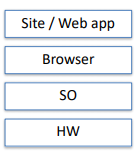
\includegraphics[width=.20\textwidth]{images/Mobile computing/7. Sviluppo/web app.PNG}
    \label{fig:sito web}
\end{figure}

Avere un'app single page non significa che c'è una sola schermata ma viene scaricata l'app con una singola chiamata al web server. 
Tramite script lato client l'utente può navigare tra più schermate senza dover ricontattare il web server. 
La web app può anche comunicare con dei web service per scambiare dati (in modo analogo a quanto fanno le app native).

Web app è una buona soluzione. La stessa web app può funzionare anche su dispositivi tradizionali.
Tra i problemi principali ci sono: 
\begin{itemize}
    \item user experience: la UX non è la stessa che su un app
    \item accesso al SO: da browser non si può accedere a diverse funzioni del SO, come ad esempio il background
    \item performance minori
    \item connessione necessaria per caricare la pagina: se si è offline non è possibile scaricare la pagina
    \item l'app realizzata non è disponibile sullo store
\end{itemize}

\subsection{Hybrid App}
Il programmatore scrive una web app (HTML, CSS, Javascript). 
La web app viene eseguita all'interno di un'app nativa che 
contiene una web view, un componente grafico nativo che contiene contenuto web. 
L’app nativa può essere generata in automatico.

\begin{figure}[!ht]
    \centering
    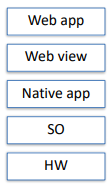
\includegraphics[width=.15\textwidth]{images/Mobile computing/7. Sviluppo/hybrid app.PNG}
    \label{fig:hybrid app}
\end{figure}

Apache Cordova è un framework molto diffuso per realizzare hybrid app. È open source.
Permette di scrivere applicazioni con tecnologie web. Permette di accedere ad alcune API del device.

PhoneGap è un framework commerciale di Adobe. 
Fornisce un'interfaccia grafica per la gestione di Apache Cordova e alcuni strumenti avanzati di sviluppo e testing. 

\subsubsection{Accesso alle funzionalità di SO}
In tutte le tecnologie di sviluppo cross-platform si pone un problema: come faccio a permettere l’accesso alle stesse funzionalità di SO alle quale si può accedere da codice nativo?

iOS e Android hanno funzionalità comune ma vi si accede in modo differente. 

\subsubsection{Accesso alle funzionalità del SO in Apache Cordova}
In realtà l’app nativa non contiene solo la web view, ma anche altre funzionalità (Service), implementate in codice nativo, che è possibile richiamare dal codice JavaScript. 

Questa cosa non può essere fatta nella web app perchè manca la componente di Service. 

\begin{figure}[!ht]
    \centering
    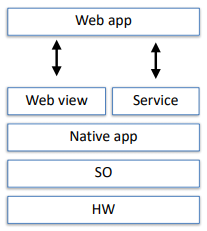
\includegraphics[width=.25\textwidth]{images/Mobile computing/7. Sviluppo/apache Cordova.PNG}
    \label{fig:apache Cordova}
\end{figure}

\subsubsection{I plugin}
In Apache Cordova esistono dei plugin che vengono distribuiti assieme al sistema. 
Possono poi essere sviluppati dei plugin aggiuntivi, ma si deve scrivere codice nativo in Android e iOS. 

In teoria, i plugin permettono di accedere a qualunque funzionalità del SO. In pratica aggiungono un livello di complessità ed obbligano il programmatore a scrivere codice nativo. In alcuni casi l'integrazione è complessa se non impossibile. 

\subsection{App ibride vs web app}
Un'app ibrida è di fatto una web app, infatti un problema che permane nelle app ibride è quello relativo alla user experience. 
L'accesso al SO viene in parte risolto con i plugin. 
Il problema delle performarce minori permane. 
Non è necessario avere la connessione per caricare la pagina e l'app realizzata è disponibile sullo store. 

\section{Conversione del codice}
Per risolvere il problema delle performance e della user experience, vogliamo fare in modo che il codice esegua come se fosse scritto in nativo. 
L'idea è di scrivere il codice una volta sola in un unico linguaggio e poi viene usato uno strumento automatico che converte questo codice in codice nativo per varie piattaforme.

Questo approccio è adottato da Xamarin.

\subsection{Xamarin}
Il programmatore scrive codice in C\#, ed ha accesso, tramite librerie di Xamarin, ad una chiamata in C\# per ogni API disponibile in Android e iOS. 
Xamarin prevede due livelli di astrazione:
\begin{itemize}
    \item livello 1: ciascuna API di SO (Android e iOS) è ri-mappata in una corrispettiva API in C\#.
    È possibile scrivere applicazioni cross-platform scrivendo una sola volta il codice che implementa la logica dell'app.
    Ogni volta che il codice interagisce con il SO, bisogna distinguere due casi, in base al SO.
    Il codice viene convertito come se fosse codice nativo. L'utente finale che vede un'app non distingue la differenza tra un pulsante creato in Xamarin e uno creato in codice nativo. 
    \\ Rimane il problema che stiamo scrivendo buona parte del codice due volte
    \item livello 2: se a livello 1 ho una chiamata per creare un pulsante in Android e un’altra chiamata per creare un pulsante in iOS, posso astrarre il concetto di pulsante e creare una chiamata che verifica la piattaforma e poi crea il pulsante corretto oppure posso applicare lo stesso approccio a tutte le principali API. Il risultato è che ho delle API di più alto livello che sono condivise per iOS e per Android
\end{itemize}

I vantaggi di Xamarin sono che il programmatore deve conoscere un unico linguaggio di programmazione, le performance elevate e la UX che è uguale a quella nativa. 
Come svantaggio si ha che tutti gli strumenti di sviluppo cross-platform aggiungono un livello di astrazione in un ambiente tecnologico e può rendere l'applicazione inutilizzabile.

\begin{figure}
    \centering
    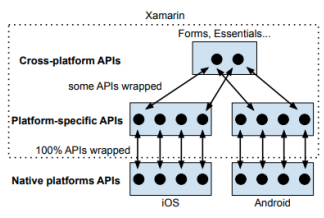
\includegraphics[width=.5\textwidth]{images/Mobile computing/7. Sviluppo/architettura Xamarin.PNG}
    \caption{Architettura Xamarin}
    \label{fig:architettura Xamarin}
\end{figure}

\subsection{Altre piattaforme di conversione}
Unity è un ambiente di sviluppo per giochi multi piattaforma. 
Si può scrivere codice in C\# o in Javascript e viene convertito per essere usato nativamente sulle varie piattaforme. 

L'altra tencologia è Flatter e le applicazioni sono scritte nel linguaggio di programmazione Dart. Il codice viene compilato in codice eseguibile per iOS e Android.
Flutter crea un contenitore dentro il quale mostra i suoi oggetti, che non sono quelli nativi. 

Un'altra tecnologia è React native che è una via di mezzo tra un sistema Hybrid e un sistema a conversione del codice.
Definiamo una GUI in HTML, ma non la mostra in una web view, ma la converte nel corrispettivo oggetto nativo. 
L’obiettivo è risolvere i problemi di UX, mediante l'uso di oggetti grafici nativi e di prestazioni, eseguendo codice nativo. 
Un problema di React native è che è basato su uno stack di librerie molto complesso e in rapida evoluzione. Basta cambiare una di queste componenti che tutto smette di funzionare. Questi non sono problemi di codice, ma sistemistici.

\subsection{La scelta della tecnologia}
La scelta di quale tecnologia di sviluppo adottare è complessa e 
richiede di considerare sia aspetti tecnici che aspetti non tecnici. \begin{itemize}
    \item Su quali piattaforme dovrà eseguire l’app? 
    \item Quali linguaggi di programmazione conosce il team di sviluppatori? 
    \item L’app dovrà eseguire anche su dispositivi tradizionali o su web? 
    \item L’app deve fare uso di funzionalità evolute di accesso alle risorse HW o SW?
\end{itemize}